% Chapter 1

\chapter{Introduction} % Main chapter title

\label{chapter1} % For referencing the chapter elsewhere, use \ref{Chapter1}

%----------------------------------------------------------------------------------------
\section{Motivation and significance}
Natural language forms the bread and butter of the legal industry, as it is expressed in contracts, judgements and legislation. The legal industry has been adopting more machine learning tools to automate and assist low level legal analysis. Worldwide legal tech market revenues were at 27.6 billion USD and is projected to to grow at a compound annual growth rate of 4\% to 35.6 billion USD by 2027 (\cite{statista}). As early as 2018, LawGeex, a contract review startup, compared the performance of lawyers vs LawGeex's machine learning model in reviewing standard template Non-Disclosure Agreements (NDA). The model beat the humans both in terms of accuracy and time, with the model having a 94\% accuracy rate and taking 26 seconds to complete the review. In comparison, the lawyers had an average accuracy of 85\% and took 92 minutes to finish the task (\cite{lawgeex}). 

Like the machine learning model that was trained by LawGeex, most legal tech tools that aim to conduct low level legal analysis use natural language processing (NLP) techniques. NLP is a branch of AI that is concerned with giving computers the ability to understand text and spoken words in much the same way human beings can (\cite{ibm_nlp}). While NLP techniques have substantially increased in performance in recent years, it has come at the cost of explainability of their predictions because of models that are architecturally more complex (\cite{zini2022}). This lack of explainability could potentially be a significant hindrance towards their adoption within the legal industry because the lawyer / law firm which uses these models still ultimately bear the legal responsibility of ensuring that the analysis is legally sound.

Nevertheless, the intersection in skillset between data science and legal analysis is still nascent and it is unrealistic to expect all legally trained personnel to be trained in data science to the extent required to interpret the predictions of machine learning models without aid. Research within the legal NLP space have focused on building higher performing models, but there have been comparatively few papers that assess the explainability of such models. At the same time, explainable AI (XAI) techniques and research have been rising in popularity since 2020 (\cite{linardatos2020}) but have not been specifically applied onto legal text. Therefore, this project aims to bridge the gap between the lawyer and the data scientist by using Explainable AI techniques to explain the predictions of machine learning models. 

For this capstone, I focus on NLP and XAI in the specific context of data privacy. While I further elaborate why I focus on data privacy in the following sections, briefly speaking, data privacy regulations have seen an increase in the need for organisations to explain the way they collect and process users' data. Therefore this context provides a realistic evaluation of the interpretability of models that are trained on legal texts relating to data privacy.

\subsection{Development and importance of explainable AI in legal technology}



\subsection{Development and importance of data privacy regulation}


\section{Explanation of the APP-350 Corpus}
The APP-350 Corpus consists of 350 annotated Android app privacy policies. Each annotation consists of a practice and a modality.

A "privacy practice" (or "practice") describes a certain behaviour of an app that can have privacy implications (e.g., collection of a phone's device identifier or sharing of its location with ad networks). There are two modalities: PERFORMED (i.e. a practice is explicitly described as being performed) and NOT\_PERFORMED (i.e. a practice is explicitly described as not being performed).

As not all practices had modalities, altogether, 57 different categories were annotated. The following is a table of the practices and their descriptions.

\begin{table}[]
	\resizebox{\textwidth}{!}{%
	\begin{tabular}{ll}
	\hline
	Data Type                 & Description                                                                                    \\ \hline
	Contact                   & The policy describes collection of unspecified contact data.                                   \\
	Contact\_Address\_Book    & The policy describes collection of contact data from a user's address book on the phone.       \\
	Contact\_City             & The policy describes collection of the user's city.                                            \\ 
	Contact\_E\_Mail\_Address & The policy describes collection of the user's e-mail.                                          \\
	Contact\_Password         & The policy describes collection of the user's password.                                        \\
	Contact\_Phone\_Number    & The policy describes collection of the user's phone number.                                    \\
	Contact\_Postal\_Address  & The policy describes collection of the user's postal address.                                  \\
	Contact\_ZIP              & The policy describes collection of the user's ZIP code.                                        \\
	Demographic               & The policy describes collection of the user's unspecified demographic data.                    \\
	Demographic\_Age          & The policy describes collection of the user's age (including birth date and age range).        \\
	Demographic\_Gender       & The policy describes collection of the user's gender.                                          \\
	Identifier                & The policy describes collection of the user's unspecified identifiers.                         \\
	Identifier\_Ad\_ID        & The policy describes collection of the user's ad ID (such as the Google Ad ID).                \\
	Identifier\_Cookie\_or\_similar\_Tech & The policy describes collection of the user's HTTP cookies, flash cookies, pixel tags, or similar identifiers. \\
	Identifier\_Device\_ID    & The policy describes collection of the user's device ID (such as the Android ID).              \\
	Identifier\_IMEI          & The policy describes collection of the user's IMEI (International Mobile Equipment Identity).  \\
	Identifier\_IMSI          & The policy describes collection of the user's IMSI (International Mobile Subscriber Identity). \\
	Identifier\_IP\_Address   & The policy describes collection of the user's IP address.                                      \\
	Identifier\_MAC           & The policy describes collection of the user's MAC address.                                     \\
	Identifier\_Mobile\_Carrier           & The policy describes collection of the user's mobile carrier name or other mobile carrier identifier.          \\
	Identifier\_SIM\_Serial   & The policy describes collection of the user's SIM serial number.                               \\
	Identifier\_SSID\_BSSID   & The policy describes collection of the user's SSID or BSSID.                                   \\
	Location                  & The policy describes collection of the user's unspecified location data.                       \\
	Location\_Bluetooth       & The policy describes collection of the user's Bluetooth location data.                         \\
	Location\_Cell\_Tower     & The policy describes collection of the user's cell tower location data.                        \\
	Location\_GPS             & The policy describes collection of the user's GPS location data.                               \\
	Location\_IP\_Address     & The policy describes collection of the user's IP location data.                                \\
	Location\_WiFi            & The policy describes collection of the user's WiFi location data.                              \\
	SSO                       & The policy describes receiving data from an unspecified single sign on service.                \\
	Facebook\_SSO             & The policy describes receiving data from the Facebook single sign on service.                 
	\end{tabular}%
	}
	\caption{List of annotated data privacy practices and their descriptions.}
	\end{table}


The APP-350 Corpus was used in a broader project to train machine learning models to conduct a privacy census of 1,035,853 Android apps. In that project, the researchers downloaded the data privacy practices of all apps from the Play Store with more than 350 million installs (which totalled 247 apps) and 103 randomly selected apps with 5 million installs. In total, the researchers collected the data privacy policies of 350 apps.

All 350 policies were annotated by one of the authors, a lawyer with experience in data privacy law. To ensure reliability of annotations, 2 other law students were hired to double annotate 10\% of the corpus. With a mean of Krippendorff's $\alpha = 0.78$\footnote{Krippendorff's $\alpha$ is a measure of agreement, with $\alpha > 0.8$ indicating good agreement, $0.67 <= \alpha <= 0.8$ indicating fair agreement, and $\alpha < 0.67$ indicating doubtful agreement.}, the agreement between the annotations exceeded previous similar research.

For more information about how the Corpus was annotated, see the paper “MAPS: Scaling Privacy Compliance Analysis to a Million Apps”, Section 3, Pg 69 to 70. 

\subsection{Rationale for utilising the APP-350 corpus}

Since the focus of this capstone is to assess the interpretability of XAI models specifically within a legal context, this dataset was chosen for the following reasons:

\begin{enumerate}
	\item APP-350 contains real-world data privacy practices as they were scraped from Google PlayStore apps. Thus training XAI models on such a dataset would provide a realistic insight into the extent of which AI models are explainable in the legal context.
	\item Legal tech companies are also using such datasets to train models as part of their contract / document review products. By using APP-350 to train XAI models, the results can be used as a (simple)\footnote{The datasets used in industry are usually much larger and the models used are more complicated. However, APP-350 would be sufficiently complicated to serve as a toy example at an undergraduate level.} proxy for the explainability of models that are currently used in the industry.
	\item APP-350 is a labelled dataset, allowing easy validation of results. If an unlabelled dataset was used, unsupervised training would have to be conducted. The performance of the models would likely be much lower because NLP models for specific vocabulary like law are still not as sophisticated as models trained on general vocabulary. Further, there are few law specific labelled datasets to begin with. 
	\item APP-350 is labelled on both the sentence and segment (i.e. paragraph) level. This provides more granular data for training the AI models. 
\end{enumerate}


\section{Problem statement}

\section{Main findings and roadmap}


\section{Font Formatting Commands}
Similarly to Word, LaTeX provides simple formatting, including \textbf{bold}, \textit{italic}, \underline{underlined} and \texttt{ugly stuff}.
However, no underline or strikethrough by default.
You can also change the size of the text, using {\tiny tiny}, {\small small}, {\large large}, {\huge huge}.
These last commands work within a specific scope.
The scope can be specified using \{ and \}, with the \{ placed before the \textbackslash{}size command.

\subsection{Special characters}
In that case, simply use \textdollar{} (by the way, note that using the dollar sign in your text switches to mathematical notation. To actually print a dollar sign use the \textbackslash{}textdollar command).
The equation above has a label, meaning you can refer to it. The numbering system uses the chapter number (in this case 1), then the equation position within the chapter (1 again).
Example: Equation~\ref{eq:eq1} is an example of an equation in LaTeX{}.
In case you would like to have an equation without numbering it? Easy!
\begin{equation*}
t = a \times log_{2}(\frac{D}{W} + 1) + b
\end{equation*}

The only difference? The \textasteriskcentered{}  symbol in the \textbackslash{}begin\{equation\textbf{\textasteriskcentered}\}.
This also works with Figures and Tables.

\section{Code Snippets}

\begin{lstlisting}
  int main (int argc, char ** argc)
  {
    printf("Hello world!\n");
    return 0;
  }
\end{lstlisting}

This template uses the \texttt{lstlisting} package, which not the best for code snippets.
However, it works without any problem, while other packages may have compatibility issues.
Feel free to try alternative solutions, the best one being \texttt{minted}.

\section{Figures}
Figures are a bit tricky with LaTeX {\tiny(not as much as tables though)}.
Let us see a simple example below:
\begin{figure}[!h]
  \centering
    
\includegraphics[width=0.9\textwidth]{figures/future.png}
  \caption{When a YNC alumni tells you that back in their days, they did not have LaTeX template and would write their report in latin on a papyrus.}
  \label{fig:future}
\end{figure}
You can refer to it: Figure~\ref{fig:future}.
This is possible thanks to the \textbackslash{}label command.
The figure should also be shown on the \hyperref[lst:figs]{List of Figures} page (note this other way of referring to another part of the manuscript!).
A common practice is use the following naming convention:
\begin{itemize}
  \item A prefix, indicating the nature of the object labelled: \texttt{eq} for equations, \texttt{fig} for figures, \texttt{tab} for tables.
  \item A colon.
  \item A unique name (easy to remember) describing your figure. Example: exp1confmatrix would suggest that the figure shows a confusion matrix for your experiment 1.
\end{itemize}

A few other points: The \textbackslash{}caption and \textbackslash{}label can be put either before or after the \textbackslash{}includegraphics command.
When you create a Figure, you need to provide placement information for LaTeX. LaTeX will usually not locate the figures \emph{exactly} where you want them.
The most common specifiers are: \texttt{h} (here), \texttt{b} (bottom of the page) and \texttt{t} (top). The \texttt{!} specifier tries to force LaTeX to put the image exactly at the location you specified (with mixed success though).
For a longer list of specifiers, please refer to: \url{https://en.wikibooks.org/wiki/LaTeX/Floats,_Figures_and_Captions}.

\subsection{Figure Size}
The size of the figure can be determined by the first parameter of the \textbackslash{}includegraphics command.
In this example, we set the size to be $0.9 \times \texttt{textwidth}$, or 90\% of the size of a column.
We could have used an absolute value in cm, e.g. \texttt{width=19cm}.

\subsection{Supported Formats}
Use standard formats, such as PNG, PDF, JPG.
LaTeX also supports other formats, such as EPS.
\textbf{Rule of thumb: use PDF as much as you can, as it uses vector graphics, making it easy to scale the figure to very large format without problems.}

\subsection{Multiple images in one figure}
You can also create complex figures with multiple images.
Here is an example, which uses a $2\times2$ layout.
The overall figure can be referred as Figure~\ref{fig:drake}.
\begin{figure}[!h]
  \begin{subfigure}[t]{.5\textwidth}
    \centering
    
\includegraphics[width=\linewidth]{figures/draketl.png}
    %\caption{We could totally insert a caption here}
    %\label{fig:draketl}
  \end{subfigure}
  \hfill
  \begin{subfigure}[t]{.5\textwidth}
    \centering
    
\includegraphics[width=\linewidth]{figures/draketr.png}
    %\caption{We could totally insert a caption here}
        %\label{fig:draketr}
  \end{subfigure}

  %\medskip
  % the medskip will have white space between both lines
  \begin{subfigure}[t]{.5\textwidth}
    \centering
    
\includegraphics[width=\linewidth]{figures/drakebl}
    %\caption{We could totally insert a caption here}
        %\label{fig:drakebl}
  \end{subfigure}
  \hfill
  \begin{subfigure}[t]{.5\textwidth}
    \centering
    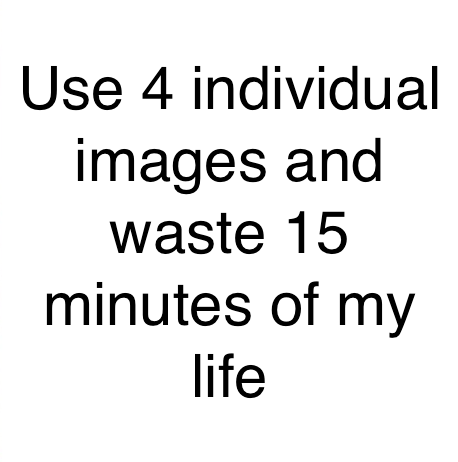
\includegraphics[width=\linewidth]{figures/drakebr}
    %\caption{We could totally insert a caption here}
    %\label{fig:drakebr}
  \end{subfigure}
  \caption{Example of a complex figures on a $2\times2$ layout.}
  \label{fig:drake}
\end{figure}

\section{Tables}
Tables can be a nightmare in LaTeX.
The easiest way to deal with tables in LaTeX is to use some online tools.
My favorite so far: \url{https://www.tablesgenerator.com/}

Here is an example of confusion matrix generated:
\begin{table}[!h]
  \resizebox{\textwidth}{!}{
\begin{tabular}{|c|c|ccccccccc}
\cline{1-2}
Chest (C)                         & -     &                                                                          &                                                                           &                                                                          &                          &                            &                           &                           &                            &                                                                            \\ \cline{1-3}
Chest (ND)  & *     & \multicolumn{1}{c|}{-}                                                   &                                                                           &                                                                          &                          &                            &                           &                           &                            &                                                                            \\ \cline{1-4}
Chest (D)   & *     & \multicolumn{1}{c|}{-}                                                   & \multicolumn{1}{c|}{*}                                                    &                                                                          &                          &                            &                           &                           &                            &                                                                            \\ \cline{1-5}
Ear          & -     & \multicolumn{1}{c|}{-}                                                   & \multicolumn{1}{c|}{-}                                                    & \multicolumn{1}{c|}{}                                                    &                          &                            &                           &                           &                            &                                                                            \\ \cline{1-6}
Thigh       & *     & \multicolumn{1}{c|}{-}                                                   & \multicolumn{1}{c|}{*}                                                    & \multicolumn{1}{c|}{*}                                                   & \multicolumn{1}{c|}{-}   &                            &                           &                           &                            &                                                                            \\ \cline{1-7}
Neck        & -     & \multicolumn{1}{c|}{*}                                                   & \multicolumn{1}{c|}{-}                                                    & \multicolumn{1}{c|}{*}                                                   & \multicolumn{1}{c|}{-}   & \multicolumn{1}{c|}{-}     &                           &                           &                            &                                                                            \\ \cline{1-8}
Palm        & -     & \multicolumn{1}{c|}{}                                                    & \multicolumn{1}{c|}{*}                                                    & \multicolumn{1}{c|}{-}                                                   & \multicolumn{1}{c|}{-}   & \multicolumn{1}{c|}{-}     & \multicolumn{1}{c|}{-}    &                           &                            &                                                                            \\ \cline{1-9}
Thumb       & -     & \multicolumn{1}{c|}{*}                                                   & \multicolumn{1}{c|}{-}                                                    & \multicolumn{1}{c|}{*}                                                   & \multicolumn{1}{c|}{-}   & \multicolumn{1}{c|}{-}     & \multicolumn{1}{c|}{*}    & \multicolumn{1}{c|}{*}    &                            &                                                                            \\ \cline{1-10}
Inner Wrist & *     & \multicolumn{1}{c|}{-}                                                   & \multicolumn{1}{c|}{-}                                                    & \multicolumn{1}{c|}{-}                                                   & \multicolumn{1}{c|}{*}   & \multicolumn{1}{c|}{*}     & \multicolumn{1}{c|}{*}    & \multicolumn{1}{c|}{-}    & \multicolumn{1}{c|}{*}     &                                                                            \\ \hline
Outer Wrist & -     & \multicolumn{1}{c|}{*}                                                   & \multicolumn{1}{c|}{-}                                                    & \multicolumn{1}{c|}{*}                                                   & \multicolumn{1}{c|}{-}   & \multicolumn{1}{c|}{-}     & \multicolumn{1}{c|}{-}    & \multicolumn{1}{c|}{*}    & \multicolumn{1}{c|}{-}     & \multicolumn{1}{c|}{-}                                                     \\ \hline
  & Belly & \multicolumn{1}{c|}{\begin{tabular}[c]{@{}c@{}}Chest\\ (C)\end{tabular}} & \multicolumn{1}{c|}{\begin{tabular}[c]{@{}c@{}}Chest\\ (ND)\end{tabular}} & \multicolumn{1}{c|}{\begin{tabular}[c]{@{}c@{}}Chest\\ (D)\end{tabular}} & \multicolumn{1}{c|}{Ear} & \multicolumn{1}{c|}{Thigh} & \multicolumn{1}{c|}{Neck} & \multicolumn{1}{c|}{Palm} & \multicolumn{1}{c|}{Thumb} & \multicolumn{1}{c|}{\begin{tabular}[c]{@{}c@{}}Inner\\ Wrist\end{tabular}} \\ \hline
\end{tabular}
}
\caption{Post-hoc comparisons between body parts. - shows no significant difference ($p>.05$), \textasteriskcentered{} shows differences ($p<.05$).}
\label{tab:posthoc}
\end{table}

Note that a table is actually a container for another type of LaTeX object, \emph{tabular}.
Tables come with captions and label, allowing us to refer to Table~\ref{tab:posthoc}.
Another interesting point is that the \textbackslash{}begin\{tabular\} command uses characters.
These characters specify how the text should be centered within each cell: \texttt{c} means centered, \texttt{l} means left and \texttt{r} means right.
Finally, my original table was too large to fit a page, so I used the \textbackslash{}resizebox\{\textbackslash{}textwidth\}\{!\}\{ command.
This command needs a closing \} after the \textbackslash{}end\{tabular\} command.
This table is also now shown in the \hyperref[lst:tabs]{List of Tables} page.
\\
\textbf{Anyway, for Tables, using the LaTeX Table Generator is a great option.}


\subsection{How to get Bibtex References?}
The easiest way to find the Bibtex snippet you need for a given reference is to use Google Scholar~(\cite{Scholar}).
On the main page, type the name of the paper you are looking for.
\\

In the results page, locate the paper:
\begin{figure}[!h]
  \centering
    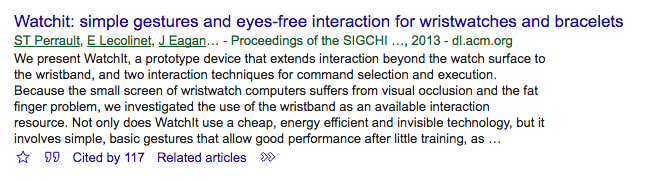
\includegraphics[width=0.9\textwidth]{figures/scholarrefexample.png}
  \caption{Example of result on Scholar}
  \label{fig:scholarref}
\end{figure}

On the last line of the result (shown in Figure~\ref{fig:scholarref}), there is a \textbf{''} symbol.
Clicking on it will display a pop-up.
\begin{figure}[!h]
  \centering
    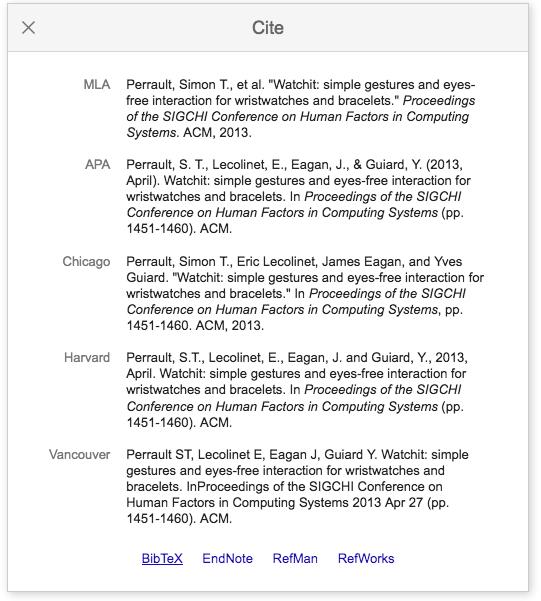
\includegraphics[width=0.7\textwidth]{figures/scholarpopup.png}
  \caption{Pop-up window with the possible citations}
  \label{fig:scholarpopup}
\end{figure}
\\

At the bottom (see Figure~\ref{fig:scholarpopup}), you will notice a ``Bibtex'' link. Click on it.
Scholar will then display a small block of text starting with @ symbol.
Copy and paste this snippet in your \texttt{biblio.bib} and you are done.
You may eventually want to check the citation key to something shorter.
\\

\textbf{You may get unexpected compilation errors with some references. The most common case is that the bibtex entry contains a DOI field, which in turn contains an underscore (\_).}
If that is the case, simply remove the DOI field (not a great practice but a good workaround).
